% this file is called up by thesis.tex
% content in this file will be fed into the main document
\chapter{Código/Manuales/Publicaciones}
\section{Distribuciones normal}


La importancia de esta distribución radica en que permite modelar numerosos fenómenos naturales. Mientras que los mecanismos que subyacen a gran parte de este tipo de fenómenos son desconocidos, por la enorme cantidad de variables incontrolables  que en ellos intervienen, el uso del modelo normal puede justificarse asumiendo que cada observación se obtiene como la suma de unas pocas causas independientes.\\

De hecho, la estadística descriptiva solo permite describir un fenómeno, sin explicación alguna. Para la explicación causal es preciso el diseño experimental, de ahí que el uso de la estadística como método correlacional.\\

La distribución normal también es importante por su relación con la estimación por mínimos cuadrados, uno de los métodos de estimación mas simples y antiguos.



\section{Señales}
Una señal es continua si no cambia de sentido o polaridad en el periodo de tiempo analizado, aún cuando se haga cero en algún, o algunos, instantes. Caso contrario es clasificado como alterna. Debemos enfatizar que estrictamente esta clasificación es independiente de la ley de variación que tenga; en la jerga técnica suele entenderse como continua a aquella que, además, es constante y como alterna aquella que, además, es senoidal simétrica, pero esto es un hecho particular.

\begin{figure}[H]
\centering
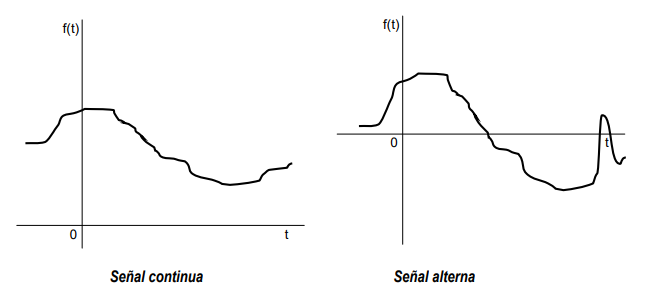
\includegraphics[width=9cm]{continua.png}
\caption{Señal continua y alterna.}
\end{figure}

La segunda clasificación es de constante o variable, siendo constante aquella que no cambia de valor ni sentido en el tiempo y variable en el caso contrario. De hecho una señal constante sólo puede ser continua aunque una continua puede ser constante o variable.\\

Dentro de las variables podemos clasificar a su vez en periódicas o en aleatorias. Periódica es aquella señal en la que puede reconocerse una ley de variación que se repite a intervalos iguales, matemáticamente podemos indicar que $f(t) = f(t+T)$ donde $T$ es el período. Aleatoria es aquella en la que no se encuentra un período de repetición. Esta clasificación es independiente del hecho de ser continua o alterna.

Para dar una idea mejor del tipo de señal a la cual nos estamos refiriendo se indica el nombre que mejor se aproxima a la forma del gráfico representativo. Así es como tenemos ondas sinodales, o armónicas, ondas cuadradas, diente de sierra, etc.

\begin{figure}[H]
\centering
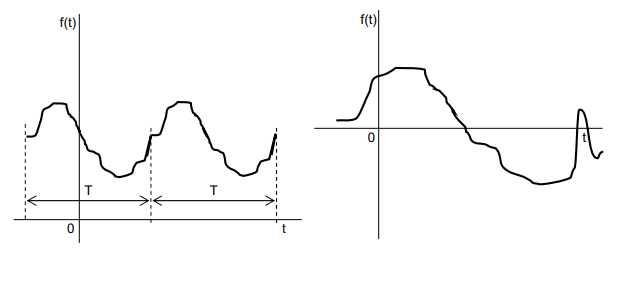
\includegraphics[width=9cm]{periodo.png}
\caption{Señal periódica y aleatorias.}
\end{figure}

\section{Apéndice}

Apéndice
